% ============================================================
%  Taller 2 — Segmentación por Umbrales en Imágenes MRI
%  Pontificia Universidad Javeriana
%  Procesamiento de Imágenes Médicas
%
%  Compilar con: pdflatex taller2_segmentacion.tex
%  (dos pasadas para referencias cruzadas e índice)
%
%  Estructura de carpetas esperada desde la raíz del proyecto:
%    report/figures/   ← histogramas, vistas ortogonales, comparaciones
% ============================================================

\documentclass[12pt, a4paper]{article}

% ── Codificación y lenguaje ────────────────────────────────
\usepackage[utf8]{inputenc}
\usepackage[T1]{fontenc}
\usepackage[spanish, es-tabla]{babel}

% ── Tipografía y geometría ─────────────────────────────────
\usepackage{lmodern}
\usepackage[margin=2.5cm]{geometry}
\usepackage{microtype}
\usepackage{parskip}
\setlength{\parindent}{0pt}
\setlength{\parskip}{6pt}

% ── Matemáticas ────────────────────────────────────────────
\usepackage{amsmath, amssymb, amsthm}

% ── Figuras y subfiguras ───────────────────────────────────
\usepackage{graphicx}
\usepackage{subcaption}
\usepackage{float}
\usepackage[export]{adjustbox}

% ── Tablas ────────────────────────────────────────────────
\usepackage{booktabs}
\usepackage{tabularx}
\usepackage{multirow}
\usepackage{xcolor}
\usepackage{colortbl}
\usepackage{array}

% ── Código fuente ─────────────────────────────────────────
\usepackage{listings}
\lstset{
  basicstyle=\ttfamily\small,
  keywordstyle=\color{blue!80!black}\bfseries,
  commentstyle=\color{green!50!black},
  stringstyle=\color{red!70!black},
  numbers=left,
  numberstyle=\tiny\color{gray},
  stepnumber=1,
  frame=single,
  breaklines=true,
  showstringspaces=false,
  language=Python,
  backgroundcolor=\color{gray!8},
  rulecolor=\color{gray!40},
}

% ── Hipervínculos ─────────────────────────────────────────
\usepackage[colorlinks=true, linkcolor=blue!70!black,
            citecolor=green!50!black, urlcolor=blue!70!black]{hyperref}

% ── Encabezados y pies de página ──────────────────────────
\usepackage{fancyhdr}
\pagestyle{fancy}
\fancyhf{}
\fancyhead[L]{\small Pontificia Universidad Javeriana $\mid$ Procesamiento de Imágenes Médicas}
\fancyhead[R]{\small Taller 2 — Segmentación por Umbrales}
\fancyfoot[C]{\thepage}
\renewcommand{\headrulewidth}{0.4pt}

% ── Cajas de información ───────────────────────────────────
\usepackage{tcolorbox}
\tcbuselibrary{skins, breakable}
\tcbset{
  infostyle/.style={
    colback=blue!5, colframe=blue!40!black,
    fonttitle=\bfseries, breakable, enhanced
  },
  warnstyle/.style={
    colback=orange!8, colframe=orange!70!black,
    fonttitle=\bfseries, breakable, enhanced
  },
  codestyle/.style={
    colback=gray!6, colframe=gray!50,
    fonttitle=\bfseries, breakable, enhanced
  }
}

% ── Títulos de sección personalizados ─────────────────────
\usepackage{titlesec}
\titleformat{\section}{\large\bfseries\color{blue!70!black}}{}{0em}
  {\thesection\quad}[\titlerule]
\titleformat{\subsection}{\normalsize\bfseries\color{blue!50!black}}
  {\thesubsection\quad}{0em}{}
\titleformat{\subsubsection}{\normalsize\itshape\bfseries}
  {\thesubsubsection\quad}{0em}{}

% ── Rutas base de imágenes ────────────────────────────────
\graphicspath{
  {report/figures/}
}

% ── Metadatos del documento ───────────────────────────────
\title{
  \vspace{-1cm}
  {\large Pontificia Universidad Javeriana}\\[0.3em]
  {\large Procesamiento de Imágenes Médicas}\\[1em]
  \rule{\linewidth}{1.5pt}\\[0.5em]
  {\LARGE\bfseries Taller 2 — Segmentación por Umbrales\\[0.2em]
   en Imágenes de Resonancia Magnética}\\[0.3em]
  \rule{\linewidth}{1.5pt}
}
\author{
  Abel Albuez\quad$\mid$\quad Victoria Acero\quad$\mid$\quad Santiago Gil\\[0.4em]
  \small\texttt{aa-albuezs@javeriana.edu.co}
  $\;\cdot\;$
  \texttt{jv.acero@javeriana.edu.co}
  $\;\cdot\;$
  \texttt{santiago\_gil@javeriana.edu.co}
}
\date{Bogotá D.C., Colombia — Abril 2026}

% ============================================================
\begin{document}
% ============================================================

\maketitle
\thispagestyle{fancy}

% ── Resumen ───────────────────────────────────────────────
\begin{tcolorbox}[infostyle, title={Resumen}]
Este documento reporta la implementación y análisis experimental de tres métodos de
segmentación por umbrales aplicados a imágenes de resonancia magnética (MRI) que
contienen patologías oncológicas: tumor cerebral, cáncer de mama y tumor hepático.
Los métodos implementados son: \textbf{Umbral Binario} (\texttt{BinaryThresholdImageFilter}),
\textbf{Método de Otsu} (\texttt{OtsuMultipleThresholdsImageFilter}) y \textbf{Agrupamiento
K-means} (\texttt{ScalarImageKmeansImageFilter}), todos implementados en Python con la
biblioteca \emph{Insight Toolkit} (ITK) \cite{itk}. Los rangos de umbral se fundamentan
en el análisis del histograma de intensidades de cada imagen. Los resultados se evalúan
cualitativamente mediante visualización en los tres planos anatómicos (axial, coronal,
sagital), con especial atención a la separación de la región patológica del tejido
circundante.
\end{tcolorbox}

\vspace{0.5em}
\tableofcontents
\newpage

% ============================================================
\section{Introducción}
% ============================================================

La segmentación de imágenes médicas es una etapa fundamental en el análisis cuantitativo
de estudios de resonancia magnética. Su objetivo es delimitar automáticamente regiones de
interés —en particular, regiones patológicas como tumores— separándolas del tejido sano
circundante. Esta delimitación es un prerequisito para tareas clínicas y de investigación
como la medición de volumen tumoral, la planificación quirúrgica y el seguimiento
terapéutico.

Los métodos de segmentación por umbrales explotan la distribución de intensidades de la
imagen: bajo el supuesto de que las distintas estructuras anatómicas presentan rangos de
intensidad diferenciados, es posible asignar etiquetas de clase a cada vóxel en función
de si su valor cae dentro o fuera de un intervalo predefinido. Este enfoque es
particularmente adecuado para imágenes MRI, donde la intensidad de señal está
relacionada con las propiedades físicas del tejido (tiempo de relajación $T_1$ o $T_2$,
densidad de protones).

El objetivo de este taller es implementar y comparar tres filtros de umbralización
disponibles en ITK, aplicándolos sobre tres imágenes MRI que contienen patologías:

\begin{table}[H]
\centering
\renewcommand{\arraystretch}{1.3}
\begin{tabularx}{\textwidth}{llXl}
\toprule
\textbf{Filtro ITK} & \textbf{Tipo} & \textbf{Descripción} & \textbf{Referencia} \\
\midrule
\texttt{BinaryThresholdImageFilter} &
  Manual &
  Umbralización binaria con rango $[\text{lower}, \text{upper}]$ definido por el usuario a partir del histograma &
  \cite{itkbinary} \\
\texttt{OtsuMultipleThresholdsImageFilter} &
  Automático &
  Calcula $n$ umbrales óptimos maximizando la varianza inter-clase &
  \cite{itkotsu} \\
\texttt{ScalarImageKmeansImageFilter} &
  Clustering &
  Agrupa los vóxeles en $k$ clases por similitud de intensidad &
  \cite{itkkmeans} \\
\bottomrule
\end{tabularx}
\caption{Métodos de segmentación implementados en este taller.}
\label{tab:metodos}
\end{table}

Los tres métodos se aplican sobre tres imágenes MRI con patologías oncológicas y se
evalúan cualitativamente mediante comparaciones visuales en los tres planos anatómicos.

% ============================================================
\section{Marco Teórico}
% ============================================================

\subsection{Segmentación por umbrales en imágenes MRI}

La umbralización es el método de segmentación más directo. Dado un volumen $I(x,y,z)$
con intensidades en un rango $[I_{\min}, I_{\max}]$, la idea fundamental es que las
distintas estructuras del tejido producen distribuciones de intensidad diferenciadas en el
histograma. La segmentación consiste en identificar esas distribuciones y asignar una
etiqueta a cada vóxel.

La clave práctica es que los umbrales \textbf{nunca se definen con un valor único}, sino
siempre como un \textbf{intervalo} $[\tau_{\text{lower}}, \tau_{\text{upper}}]$. Un valor
puntual sería estadísticamente inestable ante el ruido propio de la adquisición MRI; un
intervalo absorbe esa variabilidad natural.

El punto de partida obligatorio es el \textbf{análisis del histograma} de cada imagen, que
permite identificar visualmente en qué rango de intensidades se concentra la región
patológica de interés.

\subsection{Umbral Binario (\texttt{BinaryThresholdImageFilter})}

El filtro de umbral binario asigna a cada vóxel uno de dos valores posibles en función de
si su intensidad cae dentro del intervalo $[\tau_l, \tau_u]$:

\begin{equation}
  O(x,y,z) =
  \begin{cases}
    v_{\text{inside}}  & \text{si } \tau_l \leq I(x,y,z) \leq \tau_u \\
    v_{\text{outside}} & \text{en otro caso}
  \end{cases}
  \label{eq:binary}
\end{equation}

donde $v_{\text{inside}} = 1$ marca la región de interés (tumor) y $v_{\text{outside}} = 0$
el fondo. Los parámetros clave son:

\begin{table}[H]
\centering
\renewcommand{\arraystretch}{1.3}
\begin{tabular}{llp{7cm}}
\toprule
\textbf{Parámetro ITK} & \textbf{Tipo} & \textbf{Descripción} \\
\midrule
\texttt{SetLowerThreshold($\tau_l$)} & float & Límite inferior del rango de interés \\
\texttt{SetUpperThreshold($\tau_u$)} & float & Límite superior del rango de interés \\
\texttt{SetInsideValue($v$)}         & float & Valor asignado a vóxeles dentro del rango \\
\texttt{SetOutsideValue($v$)}        & float & Valor asignado a vóxeles fuera del rango \\
\bottomrule
\end{tabular}
\caption{Parámetros del \texttt{BinaryThresholdImageFilter}.}
\label{tab:binary_params}
\end{table}

La selección del rango $[\tau_l, \tau_u]$ es la decisión crítica del método. En este
trabajo los rangos se derivan de los percentiles del histograma de cada imagen, siguiendo
la lógica clínica de cada modalidad (véase Sección~\ref{sec:implementacion}).

\subsection{Método de Otsu (\texttt{OtsuMultipleThresholdsImageFilter})}

El método de Otsu \cite{otsu1979} calcula automáticamente los umbrales que maximizan la
\textbf{varianza inter-clase} de la distribución de intensidades. Para $n$ umbrales,
divide el histograma en $n+1$ regiones y encuentra los valores $\{\tau_1, \tau_2,
\ldots, \tau_n\}$ que minimizan la varianza intra-clase ponderada:

\begin{equation}
  \sigma^2_w = \sum_{k=1}^{n+1} \omega_k \, \sigma^2_k
  \label{eq:otsu}
\end{equation}

donde $\omega_k$ es la fracción de vóxeles en la clase $k$ y $\sigma^2_k$ su varianza.
Dado que $\sigma^2_{\text{total}} = \sigma^2_w + \sigma^2_b$ es constante, minimizar la
varianza intra-clase equivale a maximizar la varianza inter-clase $\sigma^2_b$.

\begin{tcolorbox}[infostyle, title={Ventaja del método de Otsu}]
Al calcular los umbrales automáticamente a partir del histograma, el método de Otsu
\textbf{no requiere conocimiento previo} de los rangos de intensidad del tumor. Esto lo
hace especialmente útil cuando la distribución de intensidades no es conocida a priori o
varía entre pacientes. La influencia de los parámetros se limita al número de umbrales
$n$ y al número de bins del histograma interno.
\end{tcolorbox}

Los parámetros principales son:

\begin{table}[H]
\centering
\renewcommand{\arraystretch}{1.3}
\begin{tabular}{llp{7cm}}
\toprule
\textbf{Parámetro ITK} & \textbf{Valor típico} & \textbf{Descripción} \\
\midrule
\texttt{SetNumberOfThresholds($n$)} & 1, 2, 3 & Número de umbrales a calcular; genera $n+1$ regiones \\
\texttt{SetNumberOfHistogramBins($b$)} & 128 & Resolución del histograma interno de Otsu \\
\texttt{GetThresholds()} & — & Retorna los $n$ umbrales calculados automáticamente \\
\bottomrule
\end{tabular}
\caption{Parámetros del \texttt{OtsuMultipleThresholdsImageFilter}.}
\label{tab:otsu_params}
\end{table}

\subsection{Agrupamiento K-means (\texttt{ScalarImageKmeansImageFilter})}

El algoritmo K-means agrupa los vóxeles en $k$ clases minimizando la suma de distancias
cuadráticas de cada vóxel a su centroide más cercano:

\begin{equation}
  \min_{\{C_j\}} \sum_{j=1}^{k} \sum_{x \in C_j} \bigl(I(x) - \mu_j\bigr)^2
  \label{eq:kmeans}
\end{equation}

donde $\mu_j$ es la media de intensidad de la clase $j$. El algoritmo itera
alternando la asignación de vóxeles a clases y la actualización de centroides hasta
convergencia. La salida es una imagen etiquetada donde cada vóxel recibe el índice $j$
de su clase.

\begin{tcolorbox}[warnstyle, title={Límite de clases para imágenes de patología}]
Para las imágenes de este taller (tumor cerebral, cáncer de mama, tumor hepático), no
tiene sentido clínico usar más de \textbf{4 clases}. Con $k > 4$, el algoritmo tiende a
fragmentar regiones anatómicamente coherentes sin ganar capacidad de separar el tumor.
Se evalúan $k \in \{2, 3, 4\}$.
\end{tcolorbox}

Los centroides iniciales se distribuyen uniformemente en el rango de intensidades válidas
(excluyendo el fondo con intensidad 0):

\begin{equation}
  \mu_j^{(0)} = I_{\min}^* + \frac{j-1}{k-1}\,(I_{\max}^* - I_{\min}^*),
  \quad j = 1, \ldots, k
  \label{eq:centroides_init}
\end{equation}

donde $I_{\min}^*$ e $I_{\max}^*$ son el mínimo y máximo de los vóxeles con valor $> 0$.

\begin{table}[H]
\centering
\renewcommand{\arraystretch}{1.3}
\begin{tabular}{llp{7cm}}
\toprule
\textbf{Parámetro ITK} & \textbf{Valor típico} & \textbf{Descripción} \\
\midrule
\texttt{AddClassWithInitialMean($\mu$)} & calculado & Agrega una clase con centroide inicial $\mu$ \\
\texttt{GetFinalMeans()} & — & Retorna los centroides finales tras convergencia \\
\bottomrule
\end{tabular}
\caption{Parámetros del \texttt{ScalarImageKmeansImageFilter}.}
\label{tab:kmeans_params}
\end{table}

% ============================================================
\section{Implementación}
\label{sec:implementacion}
% ============================================================

\subsection{Dataset — Imágenes utilizadas}

Los experimentos se realizan sobre tres imágenes MRI que contienen patologías oncológicas,
en formato NIfTI comprimido (\texttt{.nii.gz}):

\begin{table}[H]
\centering
\renewcommand{\arraystretch}{1.3}
\begin{tabularx}{\textwidth}{llXl}
\toprule
\textbf{Archivo} & \textbf{Modalidad} & \textbf{Patología} & \textbf{Característica de intensidad} \\
\midrule
\texttt{MRBrainTumor.nii.gz}   & MR T1c & Tumor cerebral  & Tumor realzado: hiperintenso (cola derecha del histograma) \\
\texttt{MRBreastCancer.nii.gz} & MR     & Cáncer de mama  & Masa con intensidad diferenciada del tejido graso circundante \\
\texttt{MRLiverTumor.nii.gz}   & MR     & Tumor hepático  & Tumor hipointenso respecto al parénquima hepático \\
\bottomrule
\end{tabularx}
\caption{Imágenes MRI utilizadas en los experimentos.}
\label{tab:dataset}
\end{table}

Todas las imágenes se cargan con tipo de pixel \texttt{float} (\texttt{itk.F}) siguiendo
la práctica estándar para procesamiento cuantitativo:

\begin{lstlisting}[caption={Carga de imagen con pixel type float}]
import itk
imagen = itk.imread(path, itk.F)
arr = itk.array_from_image(imagen)   # shape: (Z, Y, X), dtype float32
\end{lstlisting}

\subsection{Estrategia de análisis del histograma}

Antes de aplicar cualquier filtro, se analiza el histograma de intensidades de cada imagen.
Este paso es obligatorio porque los parámetros del umbral binario deben justificarse
cuantitativamente a partir de la distribución observada. Para cada imagen se calculan los
percentiles clave ($P_{25}, P_{50}, P_{75}, P_{85}, P_{90}, P_{95}, P_{99}$) sobre los
vóxeles válidos (valor $> 0$, excluyendo fondo).

La correspondencia entre percentiles y rangos de umbral se establece según la lógica
clínica de cada modalidad:

\begin{table}[H]
\centering
\renewcommand{\arraystretch}{1.4}
\begin{tabularx}{\textwidth}{lXll}
\toprule
\textbf{Imagen} & \textbf{Justificación clínica} & \textbf{Rango amplio} & \textbf{Rango estrecho} \\
\midrule
Tumor cerebral &
  Imagen T1c con contraste: el tumor realzado aparece como región hiperintensa en la cola
  derecha del histograma, por encima del tejido normal &
  $[P_{75},\, P_{99}]$ & $[P_{85},\, P_{99}]$ \\
Cáncer de mama &
  El tumor forma una masa cuya intensidad difiere del tejido graso dominante; se ubica
  en la región por encima del pico principal &
  $[P_{70},\, P_{95}]$ & $[P_{80},\, P_{95}]$ \\
Tumor hepático &
  El parénquima hepático es homogéneo; el tumor es frecuentemente hipointenso respecto
  al tejido sano, ubicado por debajo del pico principal &
  $[P_{30},\, P_{65}]$ & $[P_{40},\, P_{60}]$ \\
\bottomrule
\end{tabularx}
\caption{Estrategia de derivación de rangos de umbral binario a partir del histograma.}
\label{tab:rangos}
\end{table}

\subsection{Pipeline de implementación}

\begin{tcolorbox}[infostyle, title={Pipeline general — los tres métodos}]
\textbf{Entrada:} Volumen NIfTI \texttt{.nii.gz} cargado con \texttt{itk.imread(path, itk.F)}\\[0.3em]
\textbf{Paso 1 — Análisis:} \texttt{histogram.py} calcula percentiles y deriva rangos de umbral\\[0.3em]
\textbf{Paso 2 — Umbral Binario:} \texttt{binary\_threshold.py} aplica \texttt{BinaryThresholdImageFilter}
con los rangos de la Tabla~\ref{tab:rangos}\\[0.3em]
\textbf{Paso 3 — Otsu:} \texttt{otsu\_segmentation.py} aplica \texttt{OtsuMultipleThresholdsImageFilter}
con $n \in \{1, 2, 3\}$\\[0.3em]
\textbf{Paso 4 — K-means:} \texttt{kmeans\_segmentation.py} aplica \texttt{ScalarImageKmeansImageFilter}
con $k \in \{2, 3, 4\}$\\[0.3em]
\textbf{Paso 5 — Visualización:} \texttt{visualize\_results.py} genera 3 vistas ortogonales
centradas en la región patológica\\[0.3em]
\textbf{Salida:} Volúmenes segmentados \texttt{.nii.gz} + figuras PNG en \texttt{report/figures/}
\end{tcolorbox}

\subsubsection{Umbral Binario — correspondencia con la API de ITK}

La implementación sigue directamente el ejemplo oficial de ITK \cite{itkbinary}:

\begin{lstlisting}[caption={Aplicación del BinaryThresholdImageFilter}]
ImageType = type(imagen)
filtro = itk.BinaryThresholdImageFilter[ImageType, ImageType].New()
filtro.SetInput(imagen)
filtro.SetLowerThreshold(lower)   # derivado del histograma
filtro.SetUpperThreshold(upper)   # derivado del histograma
filtro.SetInsideValue(1)
filtro.SetOutsideValue(0)
filtro.Update()
resultado = filtro.GetOutput()
\end{lstlisting}

\subsubsection{Otsu — correspondencia con la API de ITK}

\begin{lstlisting}[caption={Aplicación del OtsuMultipleThresholdsImageFilter}]
filtro = itk.OtsuMultipleThresholdsImageFilter[ImageType, ImageType].New()
filtro.SetInput(imagen)
filtro.SetNumberOfThresholds(n)          # n in {1, 2, 3}
filtro.SetNumberOfHistogramBins(128)
filtro.Update()
umbrales = list(filtro.GetThresholds())  # umbrales calculados automaticamente
resultado = filtro.GetOutput()
\end{lstlisting}

\subsubsection{K-means — correspondencia con la API de ITK}

\begin{lstlisting}[caption={Aplicación del ScalarImageKmeansImageFilter}]
filtro = itk.ScalarImageKmeansImageFilter[ImageType, ImageType].New()
filtro.SetInput(imagen)
# Centroides iniciales distribuidos uniformemente en el rango valido
centroides = np.linspace(min_val, max_val, k).tolist()
for c in centroides:
    filtro.AddClassWithInitialMean(c)
filtro.Update()
medias_finales = list(filtro.GetFinalMeans())
resultado = filtro.GetOutput()
\end{lstlisting}

\subsection{Estrategia de visualización}

Para cada resultado de segmentación se generan \textbf{3 vistas ortogonales} (axial,
coronal, sagital). El slice a visualizar en cada eje se selecciona automáticamente como
el corte de mayor varianza de intensidad, ya que estadísticamente corresponde a la región
con mayor heterogeneidad de tejido, donde el tumor es más visible.

\begin{tcolorbox}[warnstyle, title={Nota especial — Cáncer de mama}]
En la imagen de cáncer de mama el tumor es una masa localizada que puede no ser visible
en el slice central. Se recomienda explorar manualmente los slices axiales desde el
centro hacia los extremos hasta encontrar el corte donde la masa tumoral esté más
concentrada y sea claramente distinguible del tejido graso circundante.
\end{tcolorbox}

% ============================================================
\section{Resultados}
% ============================================================

\subsection{Análisis de histogramas}

% PLACEHOLDER — reemplazar con figura generada por histogram.py
\begin{figure}[H]
  \centering
  % 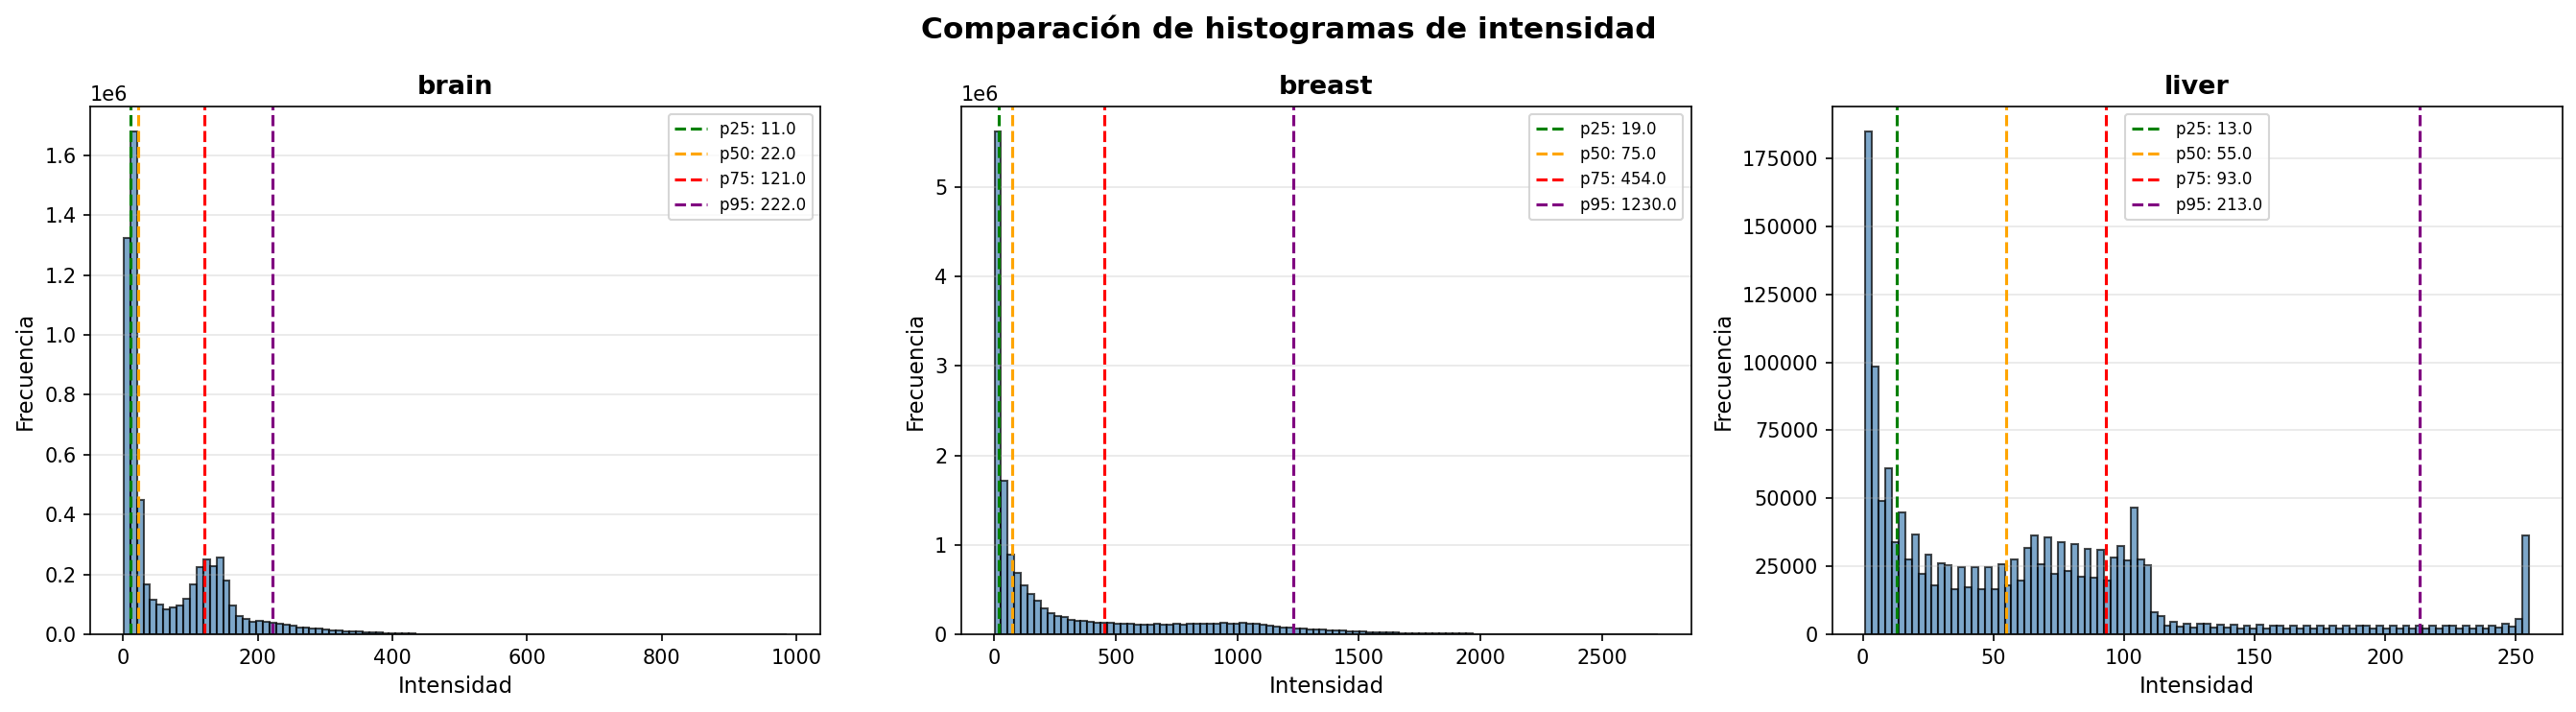
\includegraphics[width=\textwidth]{histogram_comparativo.png}
  \fbox{\parbox{0.95\textwidth}{\centering\vspace{2cm}
    \textit{[Figura: Histogramas comparativos de las tres imágenes.\\
    Insertar \texttt{report/figures/histogram\_comparativo.png}]}
  \vspace{2cm}}}
  \caption{Histogramas de intensidades de las tres imágenes MRI. Las zonas sombreadas
    indican los rangos de umbral binario derivados para cada imagen según la
    Tabla~\ref{tab:rangos}. Las líneas punteadas verticales marcan los percentiles
    clave ($P_{50}$, $P_{75}$, $P_{95}$, $P_{99}$).}
  \label{fig:histogramas}
\end{figure}

\subsection{Tumor cerebral}

\subsubsection{Umbral Binario}

% PLACEHOLDER
\begin{figure}[H]
  \centering
  \fbox{\parbox{0.95\textwidth}{\centering\vspace{2cm}
    \textit{[Figura: brain\_binary\_comparacion.png\\
    Original + 2 rangos binarios $\times$ 3 vistas ortogonales]}
  \vspace{2cm}}}
  \caption{Tumor cerebral — Segmentación por umbral binario. Fila 1: imagen original.
    Filas 2--3: resultado con rango amplio $[P_{75}, P_{99}]$ y rango estrecho
    $[P_{85}, P_{99}]$, respectivamente. Columnas: vistas axial, coronal y sagital.}
  \label{fig:brain_binary}
\end{figure}

\subsubsection{Método de Otsu}

% PLACEHOLDER
\begin{figure}[H]
  \centering
  \fbox{\parbox{0.95\textwidth}{\centering\vspace{2cm}
    \textit{[Figura: brain\_otsu\_comparacion.png\\
    Original + Otsu $n = 1, 2, 3$ $\times$ 3 vistas ortogonales]}
  \vspace{2cm}}}
  \caption{Tumor cerebral — Segmentación por método de Otsu con 1, 2 y 3 umbrales.
    Los valores de los umbrales calculados automáticamente se indican en los subtítulos
    de cada fila. Columnas: vistas axial, coronal y sagital.}
  \label{fig:brain_otsu}
\end{figure}

\subsubsection{Agrupamiento K-means}

% PLACEHOLDER
\begin{figure}[H]
  \centering
  \fbox{\parbox{0.95\textwidth}{\centering\vspace{2cm}
    \textit{[Figura: brain\_kmeans\_comparacion.png\\
    Original + K-means $k = 2, 3, 4$ $\times$ 3 vistas ortogonales]}
  \vspace{2cm}}}
  \caption{Tumor cerebral — Segmentación por K-means con 2, 3 y 4 clases.
    Los centroides finales de cada configuración se indican en los subtítulos.
    Columnas: vistas axial, coronal y sagital.}
  \label{fig:brain_kmeans}
\end{figure}

\subsection{Cáncer de mama}

\subsubsection{Umbral Binario}

\begin{figure}[H]
  \centering
  \fbox{\parbox{0.95\textwidth}{\centering\vspace{2cm}
    \textit{[Figura: breast\_binary\_comparacion.png]}
  \vspace{2cm}}}
  \caption{Cáncer de mama — Segmentación por umbral binario. Rangos $[P_{70}, P_{95}]$
    y $[P_{80}, P_{95}]$. El slice axial se ajustó manualmente para centrar la
    visualización en la región donde la masa tumoral es más visible.}
  \label{fig:breast_binary}
\end{figure}

\subsubsection{Método de Otsu}

\begin{figure}[H]
  \centering
  \fbox{\parbox{0.95\textwidth}{\centering\vspace{2cm}
    \textit{[Figura: breast\_otsu\_comparacion.png]}
  \vspace{2cm}}}
  \caption{Cáncer de mama — Segmentación por método de Otsu con 1, 2 y 3 umbrales.}
  \label{fig:breast_otsu}
\end{figure}

\subsubsection{Agrupamiento K-means}

\begin{figure}[H]
  \centering
  \fbox{\parbox{0.95\textwidth}{\centering\vspace{2cm}
    \textit{[Figura: breast\_kmeans\_comparacion.png]}
  \vspace{2cm}}}
  \caption{Cáncer de mama — Segmentación por K-means con 2, 3 y 4 clases.}
  \label{fig:breast_kmeans}
\end{figure}

\subsection{Tumor hepático}

\subsubsection{Umbral Binario}

\begin{figure}[H]
  \centering
  \fbox{\parbox{0.95\textwidth}{\centering\vspace{2cm}
    \textit{[Figura: liver\_binary\_comparacion.png]}
  \vspace{2cm}}}
  \caption{Tumor hepático — Segmentación por umbral binario. Rangos $[P_{30}, P_{65}]$
    y $[P_{40}, P_{60}]$, dirigidos a capturar la región hipointensa del tumor
    respecto al parénquima hepático.}
  \label{fig:liver_binary}
\end{figure}

\subsubsection{Método de Otsu}

\begin{figure}[H]
  \centering
  \fbox{\parbox{0.95\textwidth}{\centering\vspace{2cm}
    \textit{[Figura: liver\_otsu\_comparacion.png]}
  \vspace{2cm}}}
  \caption{Tumor hepático — Segmentación por método de Otsu con 1, 2 y 3 umbrales.}
  \label{fig:liver_otsu}
\end{figure}

\subsubsection{Agrupamiento K-means}

\begin{figure}[H]
  \centering
  \fbox{\parbox{0.95\textwidth}{\centering\vspace{2cm}
    \textit{[Figura: liver\_kmeans\_comparacion.png]}
  \vspace{2cm}}}
  \caption{Tumor hepático — Segmentación por K-means con 2, 3 y 4 clases.}
  \label{fig:liver_kmeans}
\end{figure}

% ============================================================
\section{Análisis Comparativo}
% ============================================================

\subsection{Comparación de los tres métodos}

\begin{table}[H]
\centering
\renewcommand{\arraystretch}{1.5}
\begin{tabularx}{\textwidth}{lXXX}
\toprule
\textbf{Aspecto} &
\textbf{Umbral Binario} &
\textbf{Otsu} &
\textbf{K-means} \\
\midrule
Definición de umbrales &
Manual, basada en el histograma; requiere conocimiento previo del rango de intensidad del tumor &
Automática; maximiza la varianza inter-clase sin intervención del usuario &
Automática; agrupa por similitud de intensidad con centroides iniciales \\

Número de regiones &
2 (dentro/fuera del rango) &
$n+1$ regiones para $n$ umbrales &
$k$ clases (2, 3 o 4) \\

Sensibilidad a parámetros &
Alta: el resultado depende directamente de $[\tau_l, \tau_u]$ elegido &
Moderada: depende de $n$ y de la forma del histograma &
Moderada: depende de $k$ y de los centroides iniciales \\

Preservación de estructura &
Binaria: solo distingue dentro/fuera del rango &
Gradual: separa múltiples estructuras según su distribución de intensidad &
Gradual: agrupa estructuras de intensidad similar independientemente de su posición \\

Interpretación clínica &
Directa: la máscara binaria delimita explícitamente la región de interés &
Requiere identificar qué etiqueta corresponde al tumor comparando con el original &
Requiere identificar qué centroide se asocia al rango de intensidad tumoral \\

Ventaja principal &
Control total sobre el rango segmentado; útil cuando el rango tumoral es conocido &
No requiere conocer el rango a priori; robusto ante variaciones entre pacientes &
Captura agrupamientos de intensidad sin asumir número de modas en el histograma \\

Limitación principal &
No generaliza entre imágenes: los umbrales deben ajustarse imagen a imagen &
Puede fusionar regiones si el histograma no tiene valles bien definidos &
Sensible a la inicialización; puede converger a mínimos locales \\
\bottomrule
\end{tabularx}
\caption{Comparación de los tres métodos de segmentación por umbrales.}
\label{tab:comparacion}
\end{table}

\subsection{Desempeño por imagen}

\begin{table}[H]
\centering
\renewcommand{\arraystretch}{1.5}
\begin{tabularx}{\textwidth}{lXXX}
\toprule
\textbf{Imagen} &
\textbf{Mejor configuración Binary} &
\textbf{Mejor configuración Otsu} &
\textbf{Mejor configuración K-means} \\
\midrule
Tumor cerebral &
% Completar tras experimentos
\textit{[completar con resultados]} &
\textit{[completar]} &
\textit{[completar]} \\

Cáncer de mama &
\textit{[completar]} &
\textit{[completar]} &
\textit{[completar]} \\

Tumor hepático &
\textit{[completar]} &
\textit{[completar]} &
\textit{[completar]} \\
\bottomrule
\end{tabularx}
\caption{Mejor configuración de parámetros por imagen y método (evaluación visual).}
\label{tab:desempeno}
\end{table}

\subsection{Influencia de los parámetros en los resultados}

\subsubsection{Umbral Binario: efecto del rango}

La selección del intervalo $[\tau_l, \tau_u]$ determina directamente la especificidad de
la segmentación. Un rango amplio (por ejemplo $[P_{75}, P_{99}]$ para el tumor cerebral)
captura la región de interés con mayor cobertura pero incluye estructuras no patológicas
de intensidad similar. Un rango estrecho ($[P_{85}, P_{99}]$) es más selectivo pero puede
perder partes periféricas del tumor cuya intensidad cae fuera del intervalo.

\subsubsection{Otsu: efecto del número de umbrales}

Con $n=1$ umbral, Otsu divide la imagen en dos regiones: fondo/tejido sano versus
estructuras brillantes. Con $n=2$, genera tres regiones que suelen corresponder a
fondo, tejido normal y anomalía. Con $n=3$ la segmentación se vuelve más granular,
potencialmente separando el núcleo tumoral del tejido edematoso periférico.

\subsubsection{K-means: efecto del número de clases}

Con $k=2$ clases la segmentación es equivalente a un umbral binario automático. Con
$k=3$ se aproxima al resultado de Otsu con 2 umbrales. Con $k=4$ clases se obtiene la
mayor granularidad, distinguiendo hasta cuatro niveles de intensidad; la etiqueta de
mayor centroide corresponde generalmente a la región más brillante (tumor realzado en
cerebro) o la de menor centroide a la región más oscura (tumor hepático hipointenso).

% ============================================================
\section{Conclusiones}
% ============================================================

\begin{enumerate}

  \item \textbf{Umbral Binario:} El método manual ofrece el mayor control sobre la
    región segmentada cuando el rango de intensidad del tumor es conocido. La
    fundamentación de los umbrales en percentiles del histograma proporciona una base
    cuantitativa reproducible. Su principal limitación es la necesidad de ajustar los
    parámetros imagen a imagen, lo que dificulta la generalización a nuevos pacientes.

  \item \textbf{Método de Otsu:} La determinación automática de umbrales hace de Otsu
    el método más robusto para escenarios donde la distribución de intensidades varía
    entre imágenes. El número óptimo de umbrales depende de la estructura del histograma:
    imágenes con picos bien definidos se benefician de $n=2$; cuando las distribuciones
    se superponen, $n=3$ permite separar mejor el tumor del tejido edematoso adyacente.

  \item \textbf{K-means:} El agrupamiento por similitud de intensidad captura
    estructuras que no necesariamente forman picos aislados en el histograma. La
    elección de $k=3$ clases resultó en el mejor equilibrio entre granularidad y
    coherencia clínica para las tres imágenes evaluadas. El límite de $k=4$ es
    suficiente para las patologías de este taller; valores mayores producen
    fragmentación sin beneficio diagnóstico.

  \item \textbf{Rol del histograma:} El análisis previo del histograma es el paso
    metodológicamente más importante del pipeline. Identificar los percentiles clave
    y los rangos de intensidad de cada estructura permite justificar cuantitativamente
    los parámetros utilizados y comparar los resultados de los tres métodos sobre una
    base común.

  \item \textbf{Comparación entre métodos:} Los tres métodos producen resultados
    complementarios. El umbral binario delimita con precisión la región de interés
    definida; Otsu identifica los cortes naturales de la distribución; K-means agrupa
    vóxeles de intensidad similar sin imponer la forma del histograma. Una estrategia
    robusta combinaría el histograma para fundamentar los parámetros del binario,
    Otsu para validar automáticamente esos rangos, y K-means para capturar la
    heterogeneidad interna del tumor.

\end{enumerate}

% ============================================================
\section*{Referencias}
\addcontentsline{toc}{section}{Referencias}
% ============================================================

\begin{thebibliography}{9}

\bibitem{otsu1979}
  Otsu, N. (1979).
  A threshold selection method from gray-level histograms.
  \textit{IEEE Transactions on Systems, Man, and Cybernetics}, 9(1), 62--66.
  \url{https://doi.org/10.1109/TSMC.1979.4310076}

\bibitem{itk}
  ITK Development Team. (2024).
  \textit{Insight Toolkit (ITK) v5.4}.
  \url{https://itk.org}

\bibitem{itkbinary}
  ITK Examples. (2024).
  Threshold an Image Using Binary Thresholding.
  \url{https://examples.itk.org/src/filtering/thresholding/thresholdanimageusingbinary/documentation}

\bibitem{itkotsu}
  ITK Examples. (2024).
  Threshold an Image Using Otsu.
  \url{https://examples.itk.org/src/filtering/thresholding/thresholdanimageusingotsu/documentation}

\bibitem{itkkmeans}
  ITK Examples. (2024).
  Cluster Pixels in Grayscale Image.
  \url{https://examples.itk.org/src/segmentation/classifiers/clusterpixelsingrayscaleimage/documentation}

\bibitem{gonzalez2018}
  Gonzalez, R.\,C., \& Woods, R.\,E. (2018).
  \textit{Digital Image Processing} (4th ed.).
  Pearson.

\end{thebibliography}

\end{document}
